\chapter{Design}
\label{cha:design}

Given the purpose of the game, it is important that it is both available and accessible for the user.
This means, that users can easily get to the game, that they intuitively knows how it is supposed to work, and what they have to do to win.
The challenge will be to create a game, which manages to educate, while maintaining engaging gameplay for the user.
Many ideas for this are described in \autoref{cha:analysis}.
The latter sections will describe some game design ideas, and how a solution that achieves this could look in the early stages of the design phase.\newpage

%\section{Game Environment}
\label{sec:game_environment}

Given our purpose for the game, it is important that the game seems immediately accessible to the user. This means, that the user intuitively knows have the game is supposed to work, and how success within the game can be achieved.
The challenge will then be to create a game, which manages to educate, while maintaining excitement for the user.
The following sub-sections will describe the initial design ideas, and how a solution that achieves this could look in the early stages of the design phase.

\subsection{Gameplay}

The game is intended to be a competitive \textit{'who-has-the-best-algorithm-to-solve-a-problem-on-a playing-field'} type of game.
The player will initially be in charge of a single simple biological cell with the ability to consume food on the playing field, evolve, and grow larger. The game is finished, when one player's cell has grown larger than the opponent's cell, and opponent's cell has been consumed.
There will be multiple actions available to each player's cells, for example;
\begin{itemize}
	\item Move in a given direction.
	\item Consume food.
	\item Try to consume an opponent cell
	\item Split their cell - evenly partitioning their cell and creating a copy.
\end{itemize}
%they may chose to split-up their cell - evenly partitioning their cell and creating a copy, allowing the player to control more cells on the playing field, they could move it in a given direction, they could try to attack the other player, or perhaps they go scavenging for food.
The player programs their single cell before a game begins in an easy-to-use drag-and-drop interface.

\subsection{Programming the Cell}

Programming the cell should be inviting to the user, and not be the cause of frustration due to the occurrence of peculiar programming-oriented errors, they will be tasked to dealing with.
For this reason, it is important that the interface provides the user with feedback which gives a clear understanding of when the user has combined a string of legal or illegal programming constructs.
In general terms, it is important that the user cannot make too many construction mistakes.
Otherwise the game could become a game about debugging, when it should be a game about creating the most optimized and best algorithm/cell.

\subsection{Playing Field}

The playing field is the map on which the cells compete.
It is a 2D environment, which is split up into tiles making the playing field a grid.
Splitting the map into tiles will make it easier to solve problems such as, is a given cell within attacking range of an opponent cell, or is a given cell standing on food or some other item of interest.
Doing this will limit the freedom each user has in terms of moves and gameplay, however, since cells cannot move freely in the 2D environment (a complete 360 degrees) or make exactly the decision they may want to make. 
So as a compromise to this limitation, the group decided to use hexagonal tiles, which is also used in the blockbuster game title Civilization 5.\todo{Find eventuelt den talk Sid Meier afholder omkring Hexagons i CIV 5 og hvorfor det er superr duperr}
\section{Designing the Behavior of Cells}
\label{sec:designingBehaviorCells}

The behavior of each cell is defined by the player, since it is his/her job to program the behavior \todo{ref to designing of programming interface selection}.
However, this section will focus on the standard actions that all cells can perform and how they work.
We will also discuss other possible implementations of attributes for cells, that might include strength, speed, and vision.

\subsection{Standard Actions}

%The player will initially be in charge of a single organic cell with the ability to consume red blood cells or enemy infecting cells.
The player will initially be in charge of a single organic cell with the ability to consume stars\todo{We use stars instead of red blood cells} or enemy infecting cells.
This is done automatically if a cell moves to a tile where either a star or enemy is placed.
%The red blood cells contain oxygen, which works as a nutrient to the cell, and consuming enemy cells will also work as a nutrient, but only if the enemy cell is smaller than the players cell.
The stars contain energy, which works as a nutrient to the cell, and consuming enemy cells will also work as a nutrient, but only if the energy of the enemy cell is smaller than the energy of the players cell.
%These red blood cells are placed on the playing field, see \autoref{sec:designing_playing_field}, and consuming them will allow the initial cell to grow larger/gain health, and evolve.
These stars are placed on the playing field, see \autoref{sec:designing_playing_field}, and consuming them will allow the initial cell to grow larger/gain energy, and evolve.
Evolution can be implemented by either allowing players to modify their cells while the game is played by editing their code or by splitting the cell up into two cells.
The game is finished, when one side does not have any more cells left on the board.\newline

When the cells are on the board, they use energy for every turn, so a cell with an energy level of $100$ would have an energy level of $99$ after one turn on the board regardless of the action that cell has done. The same is true for the stars, which will also decrease in energy level over time.\todo{I can not explain why this is done, but maybe someone else can}\newline

Before the cells are released onto the playing field, the player will program the initial cell in a block structure similar to that of 'Carnage Heart' and 'Kodu Game Lab'.
In this block structure, the player will have multiple actions to implement, that is available to the initial cell and all future evolutions of that cell.
These standard actions include:\newline

\verb|Move(x:steps, y:direction)| is an action that moves the cell $x$ steps in $y$ direction.
Steps can only be positive integers, and might be limited by an ability or the energy of the cells that performs the move action.
Since the playing field consists of multiple hexagonal tiles, each cell can move in six directions.
Direction is an enum type, that can have the values (TopRight, TopLeft, BottomRight, BottomLeft, Left or Right).\todo{check later}\newline

\verb|Look(x:lookingFor, y:direction, z:trigger)|\newline 

%\verb|Consume()| is a function that, if the cell is standing on a tile containing a red blood cell or a smaller enemy cell, will make the cell consume the cell and either use the oxygen in the red blood cell or the energy in the opponent cell to grow.
%The amount of oxygen in each red blood may vary and increases over time.\newline

%\verb|Attack(y:direction)| attacks the tile in the y direction. If this tile contain an enemy cell with less health than the attacking cell, then the attacking cell will consume the enemy cells health and move to that the tile, that the enemy was standing on. If the enemy has greater health than the attacking cell, the attacking cell will be consumed completely by the enemy.\newline

\verb|Split(a:energy, y:direction)| splits the cell into two cells in the $y$ direction, where the new cell get $a$ amount of energy from the splitting cell and is place on the tile in the $y$ direction from the splitting cell.
$a$ is restricted by the energy of the splitting cell, since all cells must have a minimum energy level of $1$.
If a cell is on the edge of the playing field, it is possible to split so the new cell is placed outside the playing field, which will result in the death of the newly created cell.

\section{Designing the Playing Field}
\label{sec:designing_playing_field}
As stated in the requirements section, the game will be displayed as a 2D environment instead of 3D, since the focus of this project is not on the graphical presentation of the game, but on the combination of engagin gameplay and education. However, there are still different approaches when designing the playing field. This section will focus on these approaches and argue why some solutions have been chosen over others. We will use our own game, where the player programs a cell to move around the environment to eliminate enemy cells a an example.

\subsection{Free Environment vs. Tile-styled}

When approaching the design of a 2D environment, it might be possible to design the layout as being free or limited.
In a free environment, the cell would be able to move in all 360$^{\circ}$.
This approach is seen in the game \textit{Osmos}, that is similar to our game without the programming aspect.
The player can move a cell freely in the 2D environment to eat smaller cell and each level has a specific objective.
However, the free environment approach would possibly increase the difficulty of programming the cell in contrast to a tile-styled approach to design.
Note, that by tiles we do not mean traditional tiles, such as those used in \textit{Mahjong} and \textit{Domino}, but rather games were the playing field is made by the players at the beginning of game by laying tiles with different properties.
The tile-style is known from board games, such as \textit{The Settlers of Catan} and \textit{Hive}, where both board games use hexagonal tiles.
However, tiles may not be restricted to being hexagonal, but we will discuss this later in this section.\\

Using tiles would limit the available movements of each cell into $x$ number of directions, where $x$ denotes the amount of sides on a single tile. This limiting factor would make it easier for the player to program each cell, because for example 6 movement options are much less than 360. The question is then whether the tile-styled approach would limit the player too much, making the game less engaging and too easy. However, the same question can be applied to the free environment approach.\\

We have chosen to design the playing field as a tile-styled board game, since we do not think that the limitation of tiles makes the programming of the cells too easy. It might even increase the user base, by allowing less experienced player to program cells that have a chance to defeat more experienced players. This also effects the more experienced players, since, if multiplayer is implemented, the experienced players will then face more difficult cells. We judge, that the sense of achievement when having defeated a difficult opponent is greater than when the opponent is weak and easy to defeat.\\

However, as mentioned easier, tiles can have $x$ number of sides. The next subsection will focus on how to design the tiles in terms of number of sides on each tile and whether tiles should include different properties.

\subsection{Designing the Tiles - Polygons}

Polygons are closed 2 dimensional object that have more than 2 sides. The smallest polygon in term of sides is therefore the triangle. \textit{Bizingo} is a board game that use triangle tiles, but we have not been able to find other games. It is far more common to see games that use either square or hexagonal tiles. These approach therefore both have the appeal of being more recognizable to the user. We will mainly discuss the pros and cons with square and hexagonal tiles.\\

\todo{Discuss why hex are better than square tiles}




\section{Architecture}
\label{sec:architecture}

This section will focus on the chosen architecture for our game.
There exist different architecture, but we have look at the client-server model, peer-to-peer model and model view controller as possible candidates.
We first describe our chosen architecture and then present the alternatives.

\subsection{Client-Server Model}
Our application will make use of the Client-Server model, a model that consists of two parts, a client and a server.
The basic structure of the client-server model can be seen in \autoref{fig:client-server}.

\begin{figure}[ht]
  \centering
    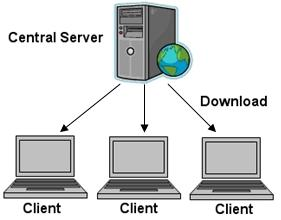
\includegraphics[width=0.5\textwidth]{img/client_server.jpg}
  \caption{Client-Server Technology \citep{ClientServer}}
  \label{fig:client-server}
\end{figure}

The client runs on the users PC, and is responsible for rendering the graphics and gameplay in the users browser.
This is done locally, without the need to connect to a server.
The client will connect to the server over the internet to receive information such as leaderboard statistics.
If multiplayer is implemented, multiple clients could be able to play against one another by connecting to a central server.
The server would then match the two or more players against each other in the same game and keep track of their individual progress.
Depending on how this is implemented, the server could also be running the clients programs.
This could be a relevant implementation for a multiple of reasons.
One reason would be to prevent cheating.
If the server executes the programs, situations where the client is modified to increase the number of points given or the time taken to solve a problem could be avoided.\todo{Other reasons?}

\subsection{Alternative Models}
\subsubsection{Peer-to-Peer}
An alternative to the Client-Server model is the Peer-to-Peer model.
The Peer-to-Peer model is like the Client-Server model without the server.
Instead all the clients connect to each other in a decentralized system, as seen in \autoref{fig:p2p}.

\begin{figure}[ht]
  \centering
    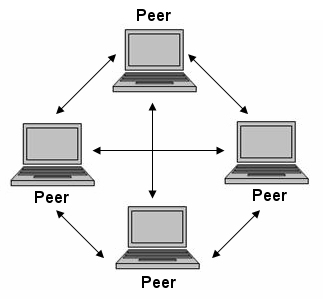
\includegraphics[width=0.4\textwidth]{img/p2p.jpg}
  \caption{Peer-to-Peer Technology \citep{PeerToPeer}}
  \label{fig:p2p}
\end{figure}

One of the positive aspects of this model is, that it drastically reduces the cost that a Client-Server based system has to keep servers running by avoiding the server completely.
However, the Peer-to-Peer model also has some negative features.
One of these features is that because most of the peers in a Peer-to-peer system are PC's, they may not always be available, and thus if no or few people are playing the game, it becomes difficult to play at all.
Another negative feature is that the prevention of cheating becomes more difficult, since it is possible to have player clients run each others programs, but modified clients can still take over the system and corrupt the results.\newline

\subsubsection{Model-View-Controller}
The Model-View-Controller design pattern separates the representation of information from a user's interaction with it.
MVC is often used in web applications and consists of three separate parts, model, view, and controller.
Due to the separation of data and user input, it is possible to have multiple different views for the same data.
An example could be that the boss of a company should be able to access a list of all employees with their salaries, where the secretary should only have access to the list of employees without salaries.
An overview of the MVC work flow can be seen on \autoref{fig:mvc}.\newline

\begin{figure}[ht]
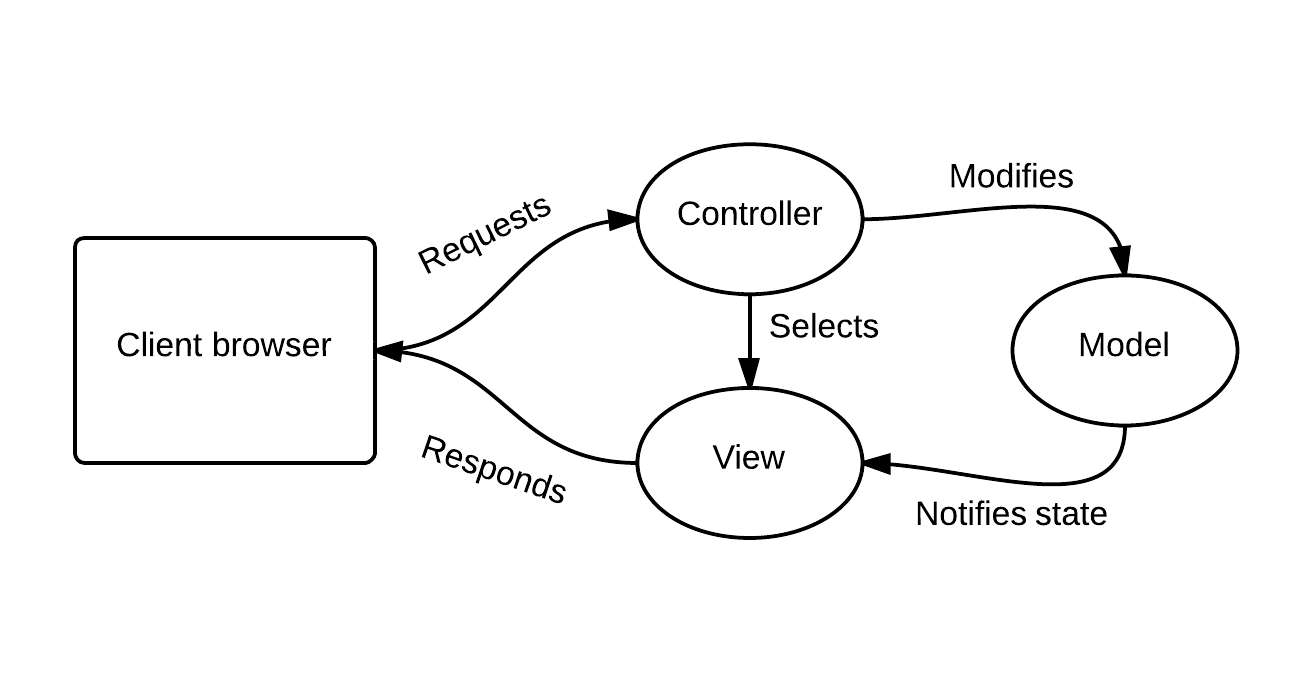
\includegraphics[width=\textwidth]{img/mvc.png}
\caption{Overview of the MVC workflow.}
\label{fig:mvc}
\end{figure}

\textbf{Model:} contains the logic, which is usually designed in such a way, that it can be reused and shared with other applications.
The model ignores how user requests are issued and how data is represented to the user.\newline

\textbf{View:} handles the representation of data for the end users.
It is possible for an application to have multiple different views for use in various situations.
The view ignores the form of user requests and the source of the data.\\

\textbf{Controller:} manages user interactions and instantiates the model and view based on performed actions, user rights and the like.
The controller ignores the logic of the model and the presentation of the view.

\todo{From Martin: You have described MVC nicely but what is the relation to your project? Why not use it in our project? (if you have not implemented it.)}
\section{Graphical Design}

Based on our analysis, it turns out that there does not seem to be a relation between the complexity of the graphics, and the impact this has on how 
much fun, the game is or how educating the game is. For this reason 2D graphics has been deemed sufficient for this game. The following section will go 
through the design choices that has been made in terms of the graphical interface of the game, along with justification for why a given choice was made.

\subsection{World Map}

The world map is a hexagon consisting of smaller 'cells' which are also hexagonal. This means that by design the entire field is hexagonal. A cell takes 
up a single small-hexagon on the field, and as does the various food types.


\begin{figure}[h]
	\centering
		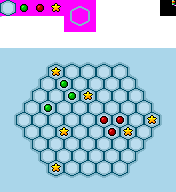
\includegraphics{img/cells_mockup.png}
	\caption{Playing field with cells and food}
	\label{fig:cells_mockup}
\end{figure}
\section{Editor Design}
\label{sec:editor_design}
Programming the cell is an essential part of the game. This is where the user will learn basic construct in the imperative paradigm by using them to program the initial cell and all future copies of that cell.

The editor is used by the player to design their program, that will be run during the game. To keep the overall design experience consistent, the editor will be using the same hexagonal design as the playing field. The programming will be done visually, and the hexagonal design will give the user more options for organizing their program.\\

The editor consists of two main parts, the programming grid of hexagons on the left, and individual fine tuning of elements on the right, an illustration can be seen on \autoref{fig:editor}.

\begin{figure}[ht]
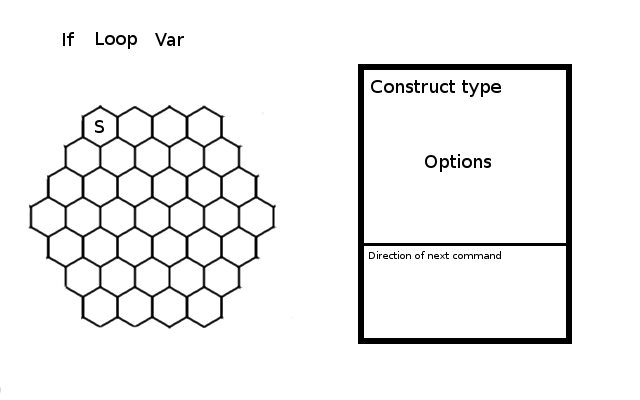
\includegraphics[width=\textwidth]{img/editor.png}
\caption{Preliminary design of the editor.}
\label{fig:editor}
\end{figure}

\subsubsection*{Programming Grid}
The programming grid makes use of a drag-and-drop interface, similar to that of the game 'Carnage Heart'.
Each programming construct, e.g. if-statements and loops, can be dragged from the top of the screen onto the hexagonal grid.
Initially this hexagonal grid only has a start point, and it is up to the player to create the program itself.
The program will be running from the start point on the grid to a user defined end point.
This end point is created by simply letting the program run outside the hexagonal grid.
By doing this, the player is essentially creating a loop, that the program will be running in during its execution.

\todo{Please check: Added from other section}It should be noted, that programming the cell should not be the cause of frustration due to the occurrence of peculiar programming-oriented errors, which the player will have to deal with.
For this reason, it is important that the interface provides the user with feedback, which gives a clear understanding of when the user has combined a string of legal or illegal programming constructs.
This can be done by implementing a basic green is correct and red is wrong color schema, that allow the user to immediately identify good code and code that includes one or more errors.
For this to work, the colors will have to be dynamic and evaluation of constructs in the program must be done on a regular basis to keep providing the player with feedback about whether the program is correct or wrong.
If the colors are not updated regularly, a construct might be flagged as red/wrong, the user corrects it, so that the construct is valid, but the construct is still flagged as red/wrong.
In general terms, it is important that the user cannot make too many construct mistakes.
Otherwise, the game is in danger of becoming a debugging game, when it should be a game about creating the most optimized and best algorithm/cell.\newline

Since the editor is using a drag-and-drop interface, adding new functionality to a program is done by dragging a construct onto the path of the current program, and define variables if needed.
Since the aim of the game is to teach programming without doing so explicitly, the variables can be define as three types/categories.
These are; numbers, entities, and directions.
The idea is that by limiting variables to three categories with meaningful names, the player will hopefully be able to easily understand what happens without prior knowledge to types in programming.
At least, this is our assumption, and if we had the time to test this, it might be possible to determine if the user would reactive positive or negative to a larger number of categories/types.

\subsubsection*{Details Panel}
The fine tuning/details panel is activated, when the player clicks on a construct, that has been placed on the hexagonal grid.
If it is deselected the fine tuning panel disappears until another construct is selected.
The panel will show different information depending on what kind of construct the player has clicked on.
For example, one of the options available for the if-statement includes a list of variables, that the if-statement can compare to generate a scenario where the variable can be in a true or false state, making the if work.
A move construct, however, will only include the option to define in which direction the cell will move.
The bottom part of the fine tuning panel is used by the player to choose, which tile on the hexagonal grid the program should be going to next.
This can be used to structure the program or make it possible for the player to customize the grid to their liking.
However, it also allows the user the freedom to create infinite loops.
Since it is NP-hard to find infinite loops in a program, we can not check the program for infinite loops for the user.
Therefore, we leave it up to the user to find these loops. 

\subsection{Design Decisions}
Several design decisions have been made for the editor.
Firstly, it was clear from the beginning, that the editor should utilize some kind of visual interface for programming, since this was used in the programming games, 'Carnage Heart' and 'Kodu Game Lab'.
If the player had to write code explicitly, it would be very clear, that the game is trying to teach programming, which goes against our goals for this project.\newline

When it was decided that the programming interface would be visual, the idea of a grid quickly became the preferred method.
As described in \autoref{sec:teachProgWithGames}, the game 'Carnage Heart' make use of a similar grid interface for programming.
It was chosen, that the editor should keep the look and feel from the game board, and thus it also makes use of a hexagonal grid.
The hexagonal grid has some features, which made preferable to a standard square grid.
The hexagonal grid makes it possible for the player to have more options as to how the program is structured.
It also makes it possible for the two branches of an if statement or a loop to be next to each other rather than on different sides of a square.\newline

The details panel was more difficult to design, since the options available are different for every construct.
Since it was decided, that the editor should utilize a visual programming interface with drag-and-drop, the player would need to be able to set some amount of variables for the program to be functional enough, such as a condition in an if-statement.
The details panel was chosen\todo{Maybe include: over what alternative}, because it removes the need to exit out of the details panel to be able to switch to the details of another construct on the grid, if the details were to pop up over the hexagonal grid.
The details panel on the right side of the hexagonal grid effectively eliminates a number of steps, with the purpose to make the game quicker and less frustrating to use.

\section{Game Rules}
\label{sec:game_rules}

This section describes the different concepts of the game, and how they interact, as well as the semantics of the various commands possible.

\subsection{Elements}

\subsubsection{Board}
The game board is a hexagonal grid inside the game world. This grid has a \emph{size}, which describes how many \emph{tiles} are along each side of the board.

\subsubsection{Position}
A position is a hexagonal segment of the game world. Each position is adjacent to 6 other positions. A position can be either inside a game board, in which case it is called a \emph{tile} or outside, which is referred to as an out of bounds, or \emph{OOB} position.

\subsubsection{Direction}
Directions describe the relation of adjacent positions. In the hexagonal grid, 6 directions exist: Left, Right, Up-Left, Up-Right, Down-Left, Down-Right.

\subsubsection{Tile}
A tile is a \emph{position} inside the game board. A tile can be either empty, or occupied by a single \emph{entity}. If two entities are inside the same position, they will \emph{battle}.

\subsubsection{OOB}
Out of bounds is the name for any positions outside the game board. Unlike \emph{tiles}, OOB positions have no concept of empty or occupied. Any entity trying to occupy an OOB position ceases to exist.

\subsubsection{Entity}
An entity is an actor in the game world. An entity can be either a \emph{cell} or \emph{food}. No matter the type of entity, they have the following properties:
\begin{itemize}
\item A \emph{position}, which they either occupy, if it is a \emph{tile}, or cease to exist if it is \emph{OOB}
\item An energy count. If this becomes zero, they cease to exist.
\end{itemize}
Each entity get a \emph{turn} in order. The turns progress in order of oldest to youngest in the game world, and then resets to the oldest again. Each entity lose one energy at the end of its turn.

\subsubsection{Food}
Food is the simplest \emph{entity}. It can take no action on its turn, and it always lose battles.

\subsubsection{Cell}
Cells are advanced \emph{entities}. In addition to the properties common to all entities, they have several more:
\begin{itemize}
\item A \emph{program}, determining its action.
\item A team, determining which other cells it considers allies, and which it considers entities.
\item A set of \emph{variables}, three of each type.
\item The instruction pointer - Information about which \emph{instruction} of of its program to start \emph{executing} from.
\end{itemize}
Apart from that a cell can take an action during its turn. It first \emph{executes} its program, then either does nothing, \emph{moves} or \emph{splits}.

\subsubsection{Program}
Like a board, a program is a hexagonal grid. Instead of tiles, the program consist of \emph{instructions}. A program can be \emph{executed}, starting from a given instruction. A program is created by a player before the game starts.

\subsubsection{Instruction}
Several instructions make up a \emph{program}. Instructions each have an \emph{instruction type} as well as several parameters pertaining to that type. When an instruction is up for execution by a program, several things may happen, according to instruction type.
\begin{itemize}
\item Variable changes - an instruction may update the values of a variable.
\item Instruction pointer update - the instruction will tell the cell which instruction to go for next.
\item Action Choice - If an instruction results in an action, the cell will take that action for the turn, and program execution will end until the next turn of that cell.
\end{itemize}
Additionally, instructions contain information about which instruction should be executed next. All instructions define a direction to \emph{continue}, while instructions representing control structures also define a direction to \emph{divert}. The chosen direction will describe to the program how to update the instruction pointer. Each instruction is described in \autoref{sub:instructions}.

\subsubsection{Variables}
Each entity has 9 variables that can be changed and read by the program. These variables are split into 3 of each three types. Each type and its domain is as follows:
\begin{itemize}
\item \emph{direction} - domain: \{ 'left' , 'right', 'up-left', 'up-right', 'down-left', 'down-right' \}
\item \emph{entitytype} - domain: \{ 'friend' , 'enemy', 'food', 'empty-tile', 'out-of-bounds' \}
\item \emph{number} - domain: $\mathbb{Z}$
\end{itemize}
Whenever an instruction needs a value of either of these types, it is possible to have it set explicitly, have it use the value stored in one of the variables, or use a derived value of the given type.

\subsubsection{Derived Values}
Derived values are values that change depending on the game state. An example of a derived value of type \emph{number} would be the cells current energy, while an example of type \emph{direction} would be the last direction the cell moved.

\subsection{Actions}

\subsubsection{No Action}
The entity does nothing. This happens when an executing program does not reach an instruction resulting in an Action Choice.

\subsubsection{Move}
The entity moves to an adjacent position, described by a \emph{direction}. If this position is occupied the moving entity will \emph{battle} the occupying entity.

\subsubsection{Split}
The entity splits into two entities. The new entity will spawn at an adjacent position, described by a \emph{direction}. Each entity will have half the energy of the original entity. In case of an uneven amount of energy, the new entity will receive the least amount. The new entity will have the same program as its parent, but will start the program from the beginning. All variables of the new entity will be set to default values. If the new entity spawned on an occupied position, it will immediately battle the occupying entity. The new entity will not get to take any action the turn it was spawned.

\subsection{Events}

\subsubsection{Battle}

Battle takes place whenever an entity (the attacker) moves to a position that is already occupied by another entity (the defender). As a position can be occupied by only one entity at a time, one of the entities must be removed. Battles happen even if the two entities are cells from the same team. The decision is made as follows:
\begin{itemize}
\item If the defender is \emph{food}, the attacker wins.
\item If the defender has less than or equal energy to the attacker, the attacker wins.
\item Else, the defender wins.
\end{itemize}
When a winner has been chosen, it receives all of the loser's energy, and the loser ceases to exist.

\subsubsection{Program Execution}

Each cell executes its program once per turn. When the program executes, it will look up an instruction depending on its current state, execute the instruction, and select the next instruction according to the \emph{divert} or \emph{continue} information of the executed instruction. This will continue until one of two things happen:
\begin{itemize}
\item It reaches an instruction resulting in an \emph{Action Choice}, in which case it tells the executing cell to perform that action.
\item It has executed an amount of instructions this turn equal to the instruction limit of 50. In this case execution is suspended for a turn and the cell is told to do nothing. This is implemented so that infinite loops without actions do not make the game impossible to complete.
\end{itemize}

\subsection{Instructions}
\label{sub:instructions}

\subsubsection{No Operation}
The no operation instruction causes no variable changes or action choices, and defines only a \emph{continue} direction.

\subsubsection{Move}
The move instruction causes an action choice. The action will be \emph{move} in a \emph{direction value}. Move defines only a \emph{continue} direction.

\subsubsection{Split}
The split instruction causes an action choice. The action will be \emph{split} in a \emph{direction value}. Split defines only a \emph{continue} direction.

\subsubsection{Look}
The look instruction causes variable changes. It will look at the position to a \emph{direction value} of the executing cell. It will store the entity type found in a chosen \emph{entitytype} variable, and the amount of energy found in a chosen \emph{number} variable. Look defines only a \emph{continue} direction.

\subsubsection{If}
The if instruction causes no variable changes or action choices. It defines a type, either \emph{entitytype}, \emph{direction} or \emph{number} as well as a boolean expression for two \emph{values} of the chosen type. Apart from the values, the expression has an operator, which for \emph{entitytype} and \emph{direction} can be either \emph{equal} or \emph{not equal}. For  \emph{number}, additional operators are available: \emph{less than}, \emph{less than or equal}, \emph{greater than} and \emph{greater than or equal}.
If defines a \emph{continue} direction for use when the expression evaluates to true, and a \emph{divert} direction for times when the expression is false.

\subsubsection{Loop}
The loop instruction causes variable changes. It defines a type, either \emph{entitytype}, \emph{direction} or \emph{number}, as well as two \emph{values} of the chosen type, called \emph{start} and \emph{end}. Additionally, it defines a loop direction depending on type. \emph{number} can be either +1 or -1. \emph{direction} can be either clockwise or counter-clockwise. \emph{entitytype} can only be a special value, \emph{nextentity}, which simply chooses the next entity type in a specified order. It also specifies a \emph{variable} of the chosen type, called the iterator. When a loop is executed, it can either be started, continued or completed, depending on the following conditions:
\begin{itemize}
\item If the loop instruction is executed for the first time in a turn, it is started.
\item If the loop is executed for the first time since it was completed, it is started.
\item If neither of the above is true and the loop is executed while the iterator is set to the end value, it is completed.
\item If it is neither started or completed, it is continued.
\end{itemize}
Loop defines both a \emph{continue} direction and a \emph{divert} direction, and acts as follows:
\begin{itemize}
\item If the loop is started, the value of the iterator is set to the start value, and the \emph{continue} direction is chosen.
\item If the loop is continued, the value of the iterator is modified by the loop direction, and the \emph{continue} direction is chosen.
\item If the loop is completed, no variable changes are made, and the \emph{divert} direction is chosen.
\end{itemize}
